\documentclass[tikz,border=8pt]{standalone}
\usepackage{tikz}
\usetikzlibrary{arrows.meta}
\begin{document}
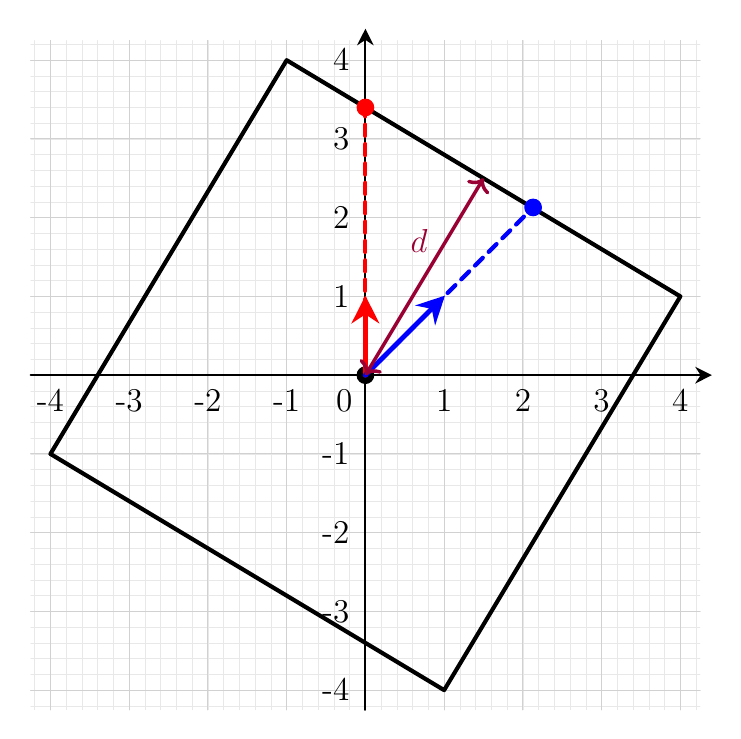
\begin{tikzpicture}[x=1.0cm,y=1.0cm,line cap=round,line join=round]
  % background grid
  \draw[step=0.2, very thin, gray!18] (-4.25,-4.25) grid (4.25,4.25);
  \draw[step=1, thin, gray!36] (-4.25,-4.25) grid (4.25,4.25);

  % square frame
  \draw[black, line width=1.5pt] (-1,4) -- (4,1) -- (1,-4) -- (-4,-1) -- cycle;

  % coordinate axes
  \draw[-{Stealth[length=6pt,width=6pt]}, black, line width=0.75pt] (-4.25,0) -- (4.4,0);
  \draw[-{Stealth[length=6pt,width=6pt]}, black, line width=0.75pt] (0,-4.25) -- (0,4.4);

  % tick labels
  \foreach \x in {-4,-3,-2,-1,1,2,3,4}{
    \node[font=\large, anchor=north] at (\x,-0.06) {\x};
  }
  \foreach \y in {-4,-3,-2,-1,1,2,3,4}{
    \node[font=\large, anchor=east] at (-0.08,\y) {\y};
  }
  \node[font=\large, anchor=north east] at (-0.04,-0.06) {0};

  \filldraw[black] (0,0) circle (3pt);

  % first vector
  \draw[-{Stealth[length=10pt,width=10pt]}, red, line width=1.75pt] (0,0) -- (0,1.01);
  \draw[red, line width=1.5pt, dash pattern=on 4pt off 3pt, dash phase=4.5pt] (0,0) -- (0,3.4);
  \filldraw[red] (0,3.4) circle (3pt);

  % second vector
  \draw[-{Stealth[length=10pt,width=10pt]}, blue, line width=1.75pt, dash phase=0pt] (0,0) -- (1.01,1.01);
  \draw[blue, line width=1.5pt, dash pattern=on 4pt off 3pt] (0,0) -- (2.13,2.13);
  \filldraw[blue] (2.13,2.13) circle (3pt);

  % length marker for vector
  \draw[<->, purple!80!black, line width=1.25pt]
    (0,0) -- (1.5,2.5);

  \node[purple!80!black, font=\large, anchor=west]
    at (0.45,1.7) {$d$};
\end{tikzpicture}
\end{document}
